\documentclass[10pt]{article}
\usepackage[utf8]{inputenc}
\usepackage[activeacute,spanish]{babel}
\usepackage[left=1.5cm,top=1.5cm,right=1.5cm, bottom=1.5cm,letterpaper, includeheadfoot]{geometry}

\usepackage{amssymb, amsmath, amsthm}
\usepackage{graphicx}
\usepackage{hyperref}
\usepackage{lmodern,url}
\usepackage{paralist} %util para listas compactas
\usepackage{xcolor}
\usepackage{bbm}
\usepackage{mathrsfs}
\usepackage{bbm}

%========PAQUETES AGREGADOS===========
%Pseudocodigo
\usepackage{pseudocode}
\usepackage[portuguese, boxruled]{algorithm2e}
\usepackage{wrapfig}
\usepackage{multicol}
\usepackage{graphicx}
\usepackage{caption}
\usepackage{subcaption}
%\captionsetup[table]{labelformat=empty}
\captionsetup[subfigure]{labelformat=empty}
\usepackage{cancel}
\usepackage{tikz}
\def\checkmark{\tikz\fill[scale=0.4](0,.35) -- (.25,0) -- (1,.7) -- (.25,.15) -- cycle;} 
%====================================

\usepackage{fancyhdr}
\pagestyle{fancy}
\fancypagestyle{plain}{%
\fancyhf{}
\lhead{\footnotesize\itshape\bfseries\rightmark}
\rhead{\footnotesize\itshape\bfseries\leftmark}
}


% macros
\newcommand{\Q}{\mathbb Q}
\newcommand{\R}{\mathbb R}
\newcommand{\N}{\mathbb N}
\newcommand{\Z}{\mathbb Z}
\newcommand{\C}{\mathbb C}
\newcommand{\BigO}{\mathcal{O}}
%Teoremas, Lemas, etc.
\theoremstyle{plain}
\newtheorem{teo}{Teorema}
\newtheorem{lem}{Lema}
\newtheorem{prop}{Proposición}
\newtheorem{cor}{Corolario}
\newtheorem{obs}{Observación}
\newtheorem{ej}{Ejemplo}
\renewcommand{\qedsymbol}{\rule{0.7em}{0.7em}}
\renewenvironment{proof}{{\bfseries \noindent Demostración}}{ \qed \\}


\theoremstyle{definition}
\newtheorem{defi}{Definición}
% fin macros


\newcommand{\catnum}{19} %numero de catedra
\newcommand{\fecha}{15 de Noviembre 2016 }

%%%%%%%%%%%%%%%%%%

%Macros para este documento
\newcommand{\cin}{\operatorname{cint}}



\begin{document}
%Encabezado
\fancyhead[L]{Facultad de Ciencias Físicas y Matemáticas}
\fancyhead[R]{Universidad de Chile}
\vspace*{-1.2 cm}
\begin{minipage}{0.6\textwidth}
\begin{flushleft}
\hspace*{-0.5cm}\textbf{MA3402-1 Estadística. Primavera 2016}\\
\hspace*{-0.5cm}\textbf{Profesor:} Raul Gouet\\
\hspace*{-0.5cm}\textbf{Escriba:} Manuel Cáceres\\
\hspace*{-0.5cm}\textbf{Fecha:} \fecha
\end{flushleft}
\end{minipage}
\begin{minipage}{0.36\textwidth}
\begin{flushright}

\includegraphics[scale=0.3]{imagenes/fcfm_dcc}
\end{flushright}
\end{minipage}
\bigskip
%Fin encabezado

\begin{center}
\LARGE\textbf{Clase \catnum}
\end{center}
\section{Modelos Lineales}
\begin{center}
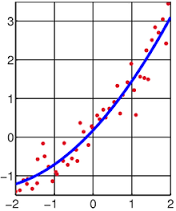
\includegraphics[scale=0.5]{imagenes/minimosCuadrados.png}
\end{center}
Tenemos puntos $(x_{i}, y_{i}), i = 1\ldots n$.\\
Estos puntos representan la respuesta ($y$) de un sistema a un estímulo ($x$).\\
Nos interesa saber como se vinculan las variables $x$ e $y$.\\
Su propósito es:
\begin{itemize}
\item Comprender el fenómeno
\item Predecir valores de $y$ no observados (inter, extra, polar)
\end{itemize}
Un típico ejemplo es el desarrollo de una función que permite calcular el volumen de madera de un árbol en función del diámetro y la altura. Aquí $y=$volumen, $x=$(diámetro,altura), es decir, la variable es bidimensional.\\

Postulamos la existencia de una función desconocida que vincula a $x$ e $y$, digamos $y_{i}=f(x_{i})$, idealmente.\\

Necesitamos una estrategia para obtener tal función o una que se acerque razonablemente.\\

\textbf{Problema:} Posiblemente no hay ninguna función si es que $x_{i}=x_{j}$ con $f(x_{i})\not = f(x_{j})$ (admito que xisten este tipo de errores), o también puede que haya infinitas de estas funciones.\\

Es necesario, antes de plantear una ``estrategia de ajuste'', reducir la clase de funciones $f$ candidatas para el modelo. Por ejemplo, restringir a funciones engendradas por una base finita, como los polinomios de grado $\le k$.\\

\section{Caso de datos en $\mathbb{R}^2$ (Mínimos cuadrados)}
Disponemos de datos $(x_{i},y_{i}), i = 1\ldots n$.\\
Buscamos $f\in \mathcal{F}$ (clase de funciones) tal que minimicen el criterio:
\begin{align*}
S(f) &= \sum_{i=1}^{n} (y_{i}-f(x_{i}))^2
\end{align*}
Resolvemos
\begin{align*}
\min_{f\in \mathcal{F}} S(f)
\end{align*}
Para comenzar, sea $\mathcal{F}$ la clase de funciones de $\mathbb{R}$ en $\mathbb{R}$ lineales afines, es decir,
\begin{align*}
\mathcal{F} &= \{f\colon \mathbb{R}\mapsto \mathbb{R} \colon f(x) = \alpha + \beta x. \alpha, \beta \in \mathbb{R}\}
\end{align*}
Con esto, el problema anterior se escribe
\begin{align*}
&\min_{\alpha, \beta \in \mathbb{R}} \underbrace{\sum_{i=1}^{n}(y_{i} - \alpha - \beta x_{i})^2}_{S(\alpha,\beta)}\\
\frac{\partial S}{\partial \alpha} &= -2\sum (y_{i} - \alpha - \beta x_{i}) = 0 \\
\frac{\partial S}{\partial \beta} &= -2\sum (y_{i} -\alpha -\beta x_{i})x_{i} = 0\\
\Rightarrow & \sum y_{i} - n\alpha - \beta\sum x_{i} = 0\\
\Rightarrow & \bar{y} = \alpha + \beta \bar{x}\\
\Rightarrow & \sum x_{i}y_{i} - \alpha\sum x_{i} - \beta\sum x_{i}^2 = 0\\
\Rightarrow & \frac{\sum x_{i}y_{i}}{n} - \alpha \bar{x} - \beta \frac{\sum x_{i}^2}{n} = 0
\end{align*}
Reemplazando $\alpha$ en la última ecuación tenemos
\begin{align*}
\frac{1}{n}  \sum x_{i}y_{i} - (\bar{y}- \beta \bar{x})\bar{x} - \beta \frac{\sum x_{i}^2}{n} = 0\\
\ldots \\
\beta = \frac{\sigma_{xy}}{\sigma_{x}^2} = \frac{\frac{1}{n}\sum x_{i}y_{i} - \bar{x}\bar{y}}{\frac{1}{n}\sum x_{i}^2 - \bar{x}^2} = \frac{\frac{1}{n}\sum (x_{i}- \bar{x})(y_{i}-\bar{y})}{\frac{1}{n}\sum (x_{i}-\bar{x})^2}
\end{align*}
Si $\sigma_{x}^2 = 0$, no hay solución sii $x_{i} = \bar{x}, \forall i = 1\ldots n$. También resulta $\hat{\alpha} = \bar{y} - \hat{\beta}\bar{x}$.\\

Hemos resuelto el sistema lineal que resulta de buscar puntos estacionarios de $S(\alpha, \beta)$. Se muestra que existe única solución cuando $\sigma_{x}>0$.\\

Aquí no tenemos ningún comentario estadístico que hacer porque no hay hipótesos probabilistica.\\

Hemos hecho un ``simple'' ajuste de mínimos cuadrados, la recta $y = \hat{\alpha} + \hat{\beta}x$ se llama recta de mínimos cuadrados es la recta más cercana a la nube en términos de distancias verticales.

\section{Hipótesos probabilísticas}
\begin{enumerate}
\item Suponemos que $x_{i}, i = 1\ldots n$ no son aleatorios.
\item Suponemos que $y_{i}, i = 1\ldots n$ provienen de variables aleatorias, es decir, cada $y_{i}$ es la realización de una variable aleatoria $Y_{i}$.
\item Supondremos que la esperanza de $Y_{i}$ depende de $X$ a través de $x_{i}$ y una función. Es decir, $\mathbb{E}(Y_{i}) = f(x_{i})$
\end{enumerate}
Se define la variable aleatoria de error $\epsilon_{i}$ como
\begin{align*}
\epsilon_{i} = Y_{i} - \mathbb{E}(Y_{i}) - Y_{i} - f(x_{i}),i = 1\ldots n
\end{align*}
tenemos $Y_{i} = f(x_{i}) + \epsilon_{i}, i = 1\ldots n$ con $\mathbb{E}(\epsilon_{i}) = 0, i = 1\ldots n$. Aparte de esto no se sabe nada de las $\epsilon_{i}$.\\

Por supuesto, hay que definir la clase $\mathcal{F}$ donde buscamos $f'$ como hicimos antes.\\

Si pensamos como en el capítulo de inferencia la búsqueda de $f\in \mathcal{F}$ se puede ver como estimación de un parámetro.\\

El espacio de parámetros aquí son $\mathcal{F}$ más los parámetros asociados a los $\epsilon_{i}$.\\

Volvamos al modelo lineal $f(x) = \alpha + \beta x$.\\

Buscamos $\alpha, \beta$ tales que se minimice
\begin{align*}
\sum_{i=1}^n (Y_{i} - \alpha - \beta X_{i})^2 = \sum_{i=1}^{n} \epsilon_{i}^2
\end{align*}
Sabemos que 
\begin{align*}
\hat{\beta} = \frac{\frac{1}{n}\sum X_{i}X_{i}- \bar{X}\bar{X}}{\frac{1}{n}\sum X_{i}^2 - \bar{X}^2} = \frac{\sigma_{XY}}{\sigma_{X}^2}
\end{align*}
Notar que $\hat{\beta}$ es una variable aleatoria función de $Y_{1},\ldots,Y_{n}$. Lo mismo pasa con $\hat{\alpha} = \bar{Y}-\hat{\beta}\bar{X}$.\\

¿Qué tan bueno son $\hat{\alpha}, \hat{\beta}$ como estimadores de $\alpha,\beta$ respectivamente?\\

Calculamos sis respectivas esperanzas
\begin{align*}
\mathbb{E}(\hat{\alpha}) &= \mathbb{E}(\bar{Y}-\hat{\beta}\bar{X})\\
&= \mathbb{Y}- \bar{X}\mathbb{E}(\hat{\beta})
\end{align*}
Sabemos que
\begin{align*}
Y_{i} &= \alpha + \beta X_{i} + \epsilon_{i}\\
\bar{Y} &= \alpha + \beta \bar{X} + \mathbb{E}(\bar{\epsilon})\\
\mathbb{E}(\bar{Y}) &= \alpha + \beta \bar{X} + \mathbb{E}(\bar{\epsilon})\\
\Rightarrow \mathbb{E}(\hat{\alpha}) &= \alpha \beta \bar{X} - \bar{X}\mathbb{E}(\hat{\beta})\\
&= \alpha + \bar{X}(\beta - \mathbb{E}(\hat{\beta}))
\end{align*}
Si $\hat{\beta}$ es insesgado para $\beta$, entonces lo mismo pasa para $\hat{\alpha}$.\\

Veamos entonces
\begin{align*}
\mathbb{E}(\hat{\beta}) &= \frac{\frac{1}{n}\sum X_{i}\mathbb{E}(Y_{i})- \bar{X}\mathbb{E}(\bar{Y})}{\sigma_{X}^2}\\
\mathbb{E}(Y_{i}) = \alpha + \beta X_{i}\\
\mathbb{E}(\bar{Y}) = \alpha + \beta \bar{X}\\
\Rightarrow \frac{1}{n}\sum X_{i}(\alpha + \beta X)  - \bar{X}(\alpha + \beta\bar{X}) = \beta \left(\frac{1}{n}\sum X_{i}^2 - \bar{X}^2\right) = \beta \sigma_{X}^2\\
\Rightarrow \mathbb{E}(\hat{\beta}) = \beta
\end{align*}
Necesitamos urgentemente conocer las varianzas de $\hat{\alpha}$ y $\hat{\beta}$ incluso sis covarianzas.\\

Por ejemplo, supongamos que los $\epsilon_{i}$ tienen varianzas finitas $\sigma_{i}^2$. Puede ser que los $\epsilon_{i},\epsilon_{j}$ estén o no correlacionados, en este caso podemos calcular las varianzas de $\hat{\alpha},\hat{\beta}$ pero las expresiones son horribles.\\

Supongamos que $Cov(\epsilon_{i},\epsilon_{j}) = \sigma_{ij}$. Entonces dado que $\hat{\beta} = \sum_{i=1}^n c_{i} Y_{i}$, se tiene que
\begin{align*}
\mathbb{V}(\hat{\beta}) &= Cov(\sum_{i=1}^n c_{i} Y_{i},\sum_{i=1}^n c_{i} Y_{i})\\
&= \sum_{i,j} c_{i}c_{j} \underbrace{Cov (Y_{i},Y_{j})}_{Cov (\epsilon_{i},\epsilon_{j})}\\
&= \sum_{i,j} c_{i}c_{j}\sigma_{ij}
\end{align*}
\end{document}